\chapter{The Large Hadron Collider}
\label{chap:lhc}
The world's foremost tool for observing physics at the electroweak scale is a particle accelerator and collider facility called the Large Hadron Collider (LHC) \cite{Breskin:1244506}. Located at the European Organization for Nuclear Research (CERN) in Geneva, Switzerland, the LHC is the largest and perhaps most complex machine ever constructed, and the source of the world's most energetic laboratory-prepared particles. This machine offers our best chance of observing evidence of new structure that may describe our universe at the smallest scales, including perhaps the particles and fields of \SUSY.

\section{LHC key features}
The primary feature of the LHC is a meter-wide, 26.7 kilometer-long cryogenic vacuum cylinder forming a nearly circular path below ground in France and Switzerland. The LHC ring occupies a 4 meter-wide tunnel whose depth ranges between 45 and 170 meters beneath the surface. During normal operation, the LHC ring houses two counter-circulating beams of energetic protons, which are steered by superconducting magnets and brought to intersect at various points around the ring. There are four such crossing points, located at the centers of the four LHC experiments, ATLAS, ALICE, CMS, and LHC-b, where high energy protons collide. The layout of the LHC is shown in Figure \ref{fig:LHCLayout}. 

\begin{figure}[t]
\centering
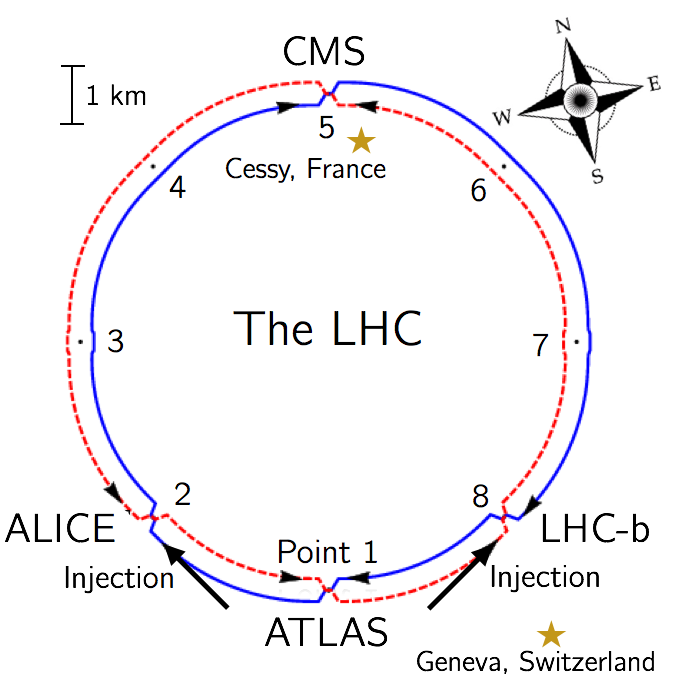
\includegraphics[width=.75\linewidth]{figures/LHC/LHC.png}
\caption{The layout of the Large Hadron Collider. The scale is approximate and the separation between the beams has been exaggerated to show the crossings of beam 1 (blue) and beam 2 (red) at interaction points 1, 2, 5, and 8.} 
\label{fig:LHCLayout}
\end{figure}

The LHC ring does not form a perfect circle, but rather is made of alternating curved and straight sections. The curved sections are 2500 meters long in arc length and are instrumented with superconducting dipole magnets. The straight sections are 530 meters long, and their centers (labeled as points 1-8 in Figure \ref{fig:LHCLayout}) have either been instrumented with hardware that serves necessary functions for the operation of the LHC, or with of the experimental facilities. 

The hardware and functionality of each of the LHC's eight points is summarized in Table \ref{tab:LHCPoints}.  The primary experimental facilities, mentioned above, observe high energy proton and heavy ion collisions and perform both standard model measurements and searches for BSM physics. In addition to the four primary experiments, Table \ref{tab:LHCPoints} lists in parentheses a few additional experimental facilities that share interaction points with the primary four. TOTEM shares the experimental cavern with CMS on the LHC ring at point 5 and measures, among other observables, proton-proton elastic scattering cross sections; MOEDAL shares the interaction point 8 with LHC-b and performs searches for particles with magnetic monopole moments, and LHC-f is a future experiment that will share interaction point 1 with ATLAS and study particles that travel nearly parallel with the beam direction (the forward direction).


\begin{table}
\begin{centering}
\caption{The hardware at the interaction points of the LHC.}
\begin{tabularx}{\textwidth}{>{\setlength\hsize{0.11\hsize}\setlength\linewidth{\hsize}}X|>{\setlength\hsize{.45\hsize}\setlength\linewidth{\hsize}}X|>{\setlength\hsize{.7\hsize}\setlength\linewidth{\hsize}}X}
\hline
\hline
point & hardware & functionality \\
\hline
\vspace{-3.00mm} 1 & \vspace{-3.00mm} ATLAS experiment \cite{Aad:2012naa}& 
\vspace{-6.5mm}
\begin{itemize}
\item full coverage particle detector
\item proton-proton collisions
\item standard model measurements and searches for evidence of new particles
\end{itemize}\\
&\vspace{-4mm}LHC-f experiment \cite{Adriani:2008zz}&
\vspace{-7mm}
\begin{itemize}
\item forward particle detector
\end{itemize}\\
\hline
\vspace{-3.00mm} 2 & \vspace{-3.00mm} ALICE experiment \cite{Leistam:644017}& 
\vspace{-6.5mm}
\begin{itemize}
\item partial coverage particle detector
\item heavy ion collisions
\end{itemize}\\
\hline
\vspace{-3.00mm} 3 & \vspace{-3.00mm} RF cavities & 
\vspace{-6.5mm}
\begin{itemize}
\item momentum cleaning
\end{itemize}\\
\hline
\vspace{-3.00mm} 4 & \vspace{-3.00mm} sextupole magnets & 
\vspace{-6.5mm}
\begin{itemize}
\item acceleration
\end{itemize}\\
\hline
\vspace{-3.00mm} 5 & \vspace{-3.00mm} CMS experiment \cite{Chatrchyan:2008aa}& 
\vspace{-6.5mm}
\begin{itemize}
\item full coverage particle detector
\item proton-proton collisions
\item standard model measurements and searches for new particles
\end{itemize}\\
\vspace{-0.0cm}
&\vspace{-4mm}TOTEM  experiment \cite{Anelli:2008zza}&
\vspace{-7mm}
\begin{itemize}
\item forward particle detector
\end{itemize}\\
\hline
\vspace{-3.00mm} 6 & \vspace{-3.00mm} quadrupole magnets & 
\vspace{-6.5mm}
\begin{itemize}
\item beam focusing
\end{itemize}\\
\hline
\vspace{-3.00mm} 7 & \vspace{-3.00mm} sextupole magnets & 
\vspace{-6.5mm}
\begin{itemize}
\item betatron cleaning
\end{itemize}\\
\hline
\vspace{-3.00mm} 8 & \vspace{-3.00mm} LHC-b experiment \cite{Alves:2008zz}& 
\vspace{-6.5mm}
\begin{itemize}
\item partial coverage particle detector
\item heavy ion collisions
\end{itemize}\\
&\vspace{-4mm}\small MOEDAL\normalsize~experiment~\cite{Pinfold:2015laa}&
\vspace{-7mm}
\begin{itemize}
\item forward physics
\end{itemize}\\
\hline
\hline
\end{tabularx}
\label{tab:LHCPoints}
\end{centering}
\end{table}

Figure \ref{fig:BeamCS} shows a typical cross section of the LHC ring. Within the outer steel casing are not only the two proton beams, but also the magnets and other instrumentation required to control and manipulate the beams. A continuous ultra high vacuum is maintained in the outer volume in order to thermally insulate the inner volume. The inner volume is filled with an iron yoke and held at a temperature of 1.9 K by supercooled liquid helium, which flows through the heat exchanger pipe. Inside the yoke and in thermal equilibrium with the iron is a twin bore assembly of niobium titanium superconducting coils that produce magnetic fields with strengths of up to 9 Tesla (T). Within the focus of the coils are the two parallel evacuated beam pipes, highways for subatomic particles.


\begin{figure}[t]
\centering
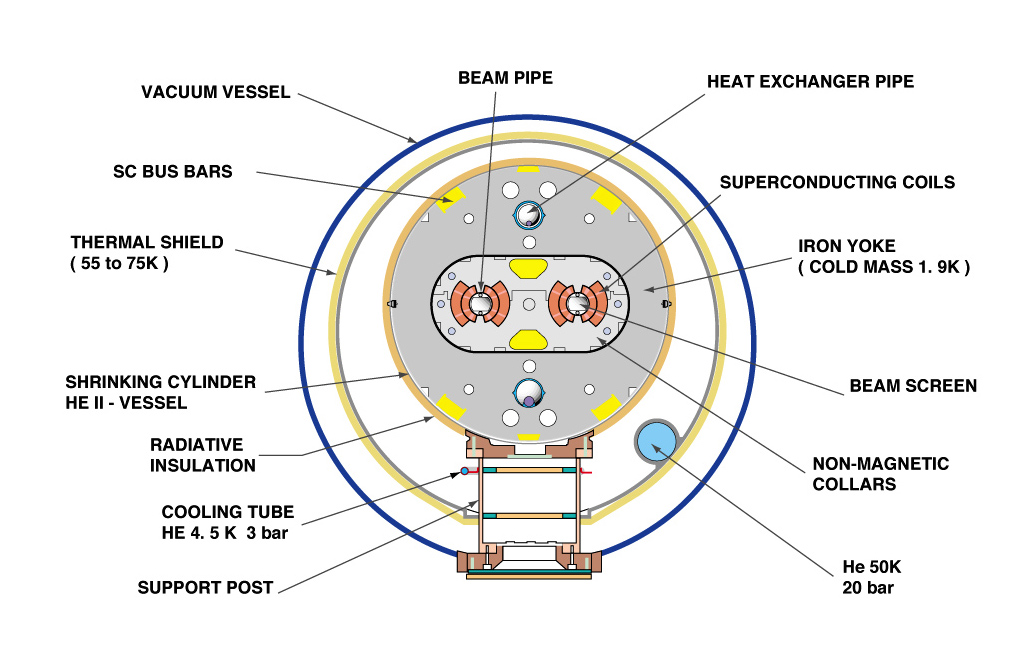
\includegraphics[width=1.0\linewidth]{figures/LHC/LHCDipole.jpg}
\caption{Cross section of a cryodipole, the most common segment of the LHC \cite{Jean-Luc:841539}. } 
\label{fig:BeamCS}
\end{figure}


The LHC's superconducting coils produce various magnetic field geometries to serve different functions. About 1200 cryodipole magnets are positioned in the curved LHC segments and produce dipole fields that bend the protons along their arched trajectories;  about 400 magnets located in the LHC's short straight sections produce quadrupole fields that are used to focus the beams, and thousands of additional magnets produce sextupole, octopole and decapole fields that purify and adjust the beams in various ways. 

Additional systems are responsible for the refrigeration of liquid helium, the powering and protection of the superconducting coils, and the maintenance and dumping of the particle beams. 

\section{The injection sequence}
Long before they reach the LHC beam pipes, protons are accelerated and focused by a multi-staged process. Initially the protons are stored as the nuclei of gaseous hydrogen atoms, kept in a sealed bottle at the CERN accelerator complex. When the LHC operators begin the procedure of filling the machine with protons, the hydrogen in the bottle is injected into a duoplasmatron~\cite{Breskin:1244506}, which subjects the hydrogen to an electric field and a bombardment of electrons. The electrons ionize the hydrogen atoms, and the electric field carries the liberated hydrogen nuclei (protons) through the duoplasmatron cavity, providing them with 100 keV of kinetic energy. Upon leaving the duoplasmatron, the protons are gathered by a quadrupole magnet and guided into the aperture of a linear accelerator called LINAC2, where they are accelerated by radio frequency (RF) cavities up to an energy of 50 MeV. LINAC2 discharges the protons into a cyclotron called the Proton Synchrotron Booster (PSB), which accelerates the protons repeatedly as they cycle around a 20-meter circular path. After reaching an energy of 1.4 GeV within the PSB, the protons are injected into a larger cyclotron called the Proton Synchrotron (PS). The PS elevates the protons' kinetic energy to 25 GeV before passing them to the world's second largest particle accelerator, the Super Proton Synchrotron (SPS), which takes the protons up to an energy of 450 GeV. The energy is now high enough for the protons to be injected into the LHC. 

Protons are injected into the LHC at 450 GeV and accelerated up to the highest energy ever achieved at a laboratory, 6.5 TeV. The beams are collided head-on, yielding a collision energy of 13 TeV in the proton-proton center of mass frame. To understand why it is necessary to push the energy frontier in this way, it is necessary to explain the goals of the LHC.


\section{The goals of the LHC}
One of the goals of the LHC is to produce and observe new, heavy particles in the collisions of protons. This of course assumes that such particles actually exist. Assuming they exist, and for concreteness, that the new particles are the particles of \SUSY, there are two main ingredients required to produce \susy~particles, both of which can be understood by examining the expression that governs how many proton-proton collisions are expected to result in the creation of \susy~particles:
\begin{equation}
N_{\rm SUSY} = \lumi\cdot \sigma_{\rm SUSY}.
\end{equation}
Here, $N_{\rm SUSY}$ is the number of events in which \susy~particles are present, where ``event'' is defined as the collection of particles emanating from a single collision. The quantity $\sigma_{\rm SUSY}$ is the interaction cross section, a measure of the probability for a supersymmetric interactions to occur during a collision. The symbol $\lumi$ stands for the integrated luminosity, and is a measure of the total number of protons collided:
\begin{equation}
\lumi = \frac{N_{\rm collisions}}{\sigma_{\rm pp}}.
\end{equation} 
Here, $N_{\rm collisions}$ is the total number of collisions achieved at the LHC and $\sigma_{\rm pp}$ is the cross section for protons to interact. Clearly, since the goal is to maximize $N_{\rm SUSY}$, it is important to maximize both $\sigma_{\rm SUSY}$ and $\lumi$. The maximization of $\sigma_{\rm SUSY}$ is achieved by imparting as much kinetic energy as possible to the protons.  The maximization of $\lumi$ is achieved by making the beam intensities, i.e., the number of protons per unit volume and time as possible. A few details on these two objectives are now given.

\subsection{The objective of high energy}

Owing to energy conservation, the probability of producing a supersymmetric particle gets lower as the hypothetical mass of the particle increases.  However, this limitation can be overcome by increasing the energy of the colliding protons. In other words, $\sigma_{\rm SUSY}$, and thus $N_{\rm SUSY}$, increase as a function of the proton energy. This is why the primary objective of the LHC is to achieve high energy collisions.


\subsection{The objective of high luminosity}
While high energy is the primary goal of the LHC, the other essential goal is to provide as large a beam intensity as possible. This is achieved by maximizing $N_{\rm collisions}$, by colliding as many protons as possible within a given period of time. To this end, the proton beams are not continuous beams, but are segmented into bunches, which are groups of a few billion protons, where the bunches are spaced apart in time intervals of 50 ns (25 ns) in Run 1 (Run 2). Maximizing the number of observed collisions is important because new physics processes are expected to be very rare, and as few as one in 10 billion collisions might contain the kind of new physics that is being looked for. The design luminosity of the LHC is $\mathcal{L}=10^{34}$ cm$^{-2}$s$^{-1}$.

